\chapter{Revisión Crítica de la Literatura}

En el presente capítulo comenzaremos discutiendo sobre un trabajo que optimiza un \emph{splitter}.
Seguidamente, identificaremos dos inconvenientes con este trabajo e iremos mostrando como otras 
investigaciones han afrontado estos desafíos.

En \cite{Prosopio-Galarza2019} se optimizó un \emph{splitter} con guías de onda fijas de altura $0.5 \mu m$, 
donde las guías de onda de salida son separadas por $0.2 \mu m$ y 
todas estas son unidas con una región rectangular de diseño de $2 \mu m \times 1.5 \mu m$.
El diseño utiliza un espesor estándar de $220 nm$.
Con esta geometría se simulan distintos diseños dividiendo la región rectangular en ($z = 13$) segmentos
uniformemente separados.
Cada segmento puede variar su altura dentro del rectángulo, estos se centran de forma vertical y
se van uniendo sus extremos. 
La representación de esta idea la podemos observar en la \autoref{fig:roy-mmi} con $z = 5$ segmentos.

\begin{figure}[ht]
  \centering
  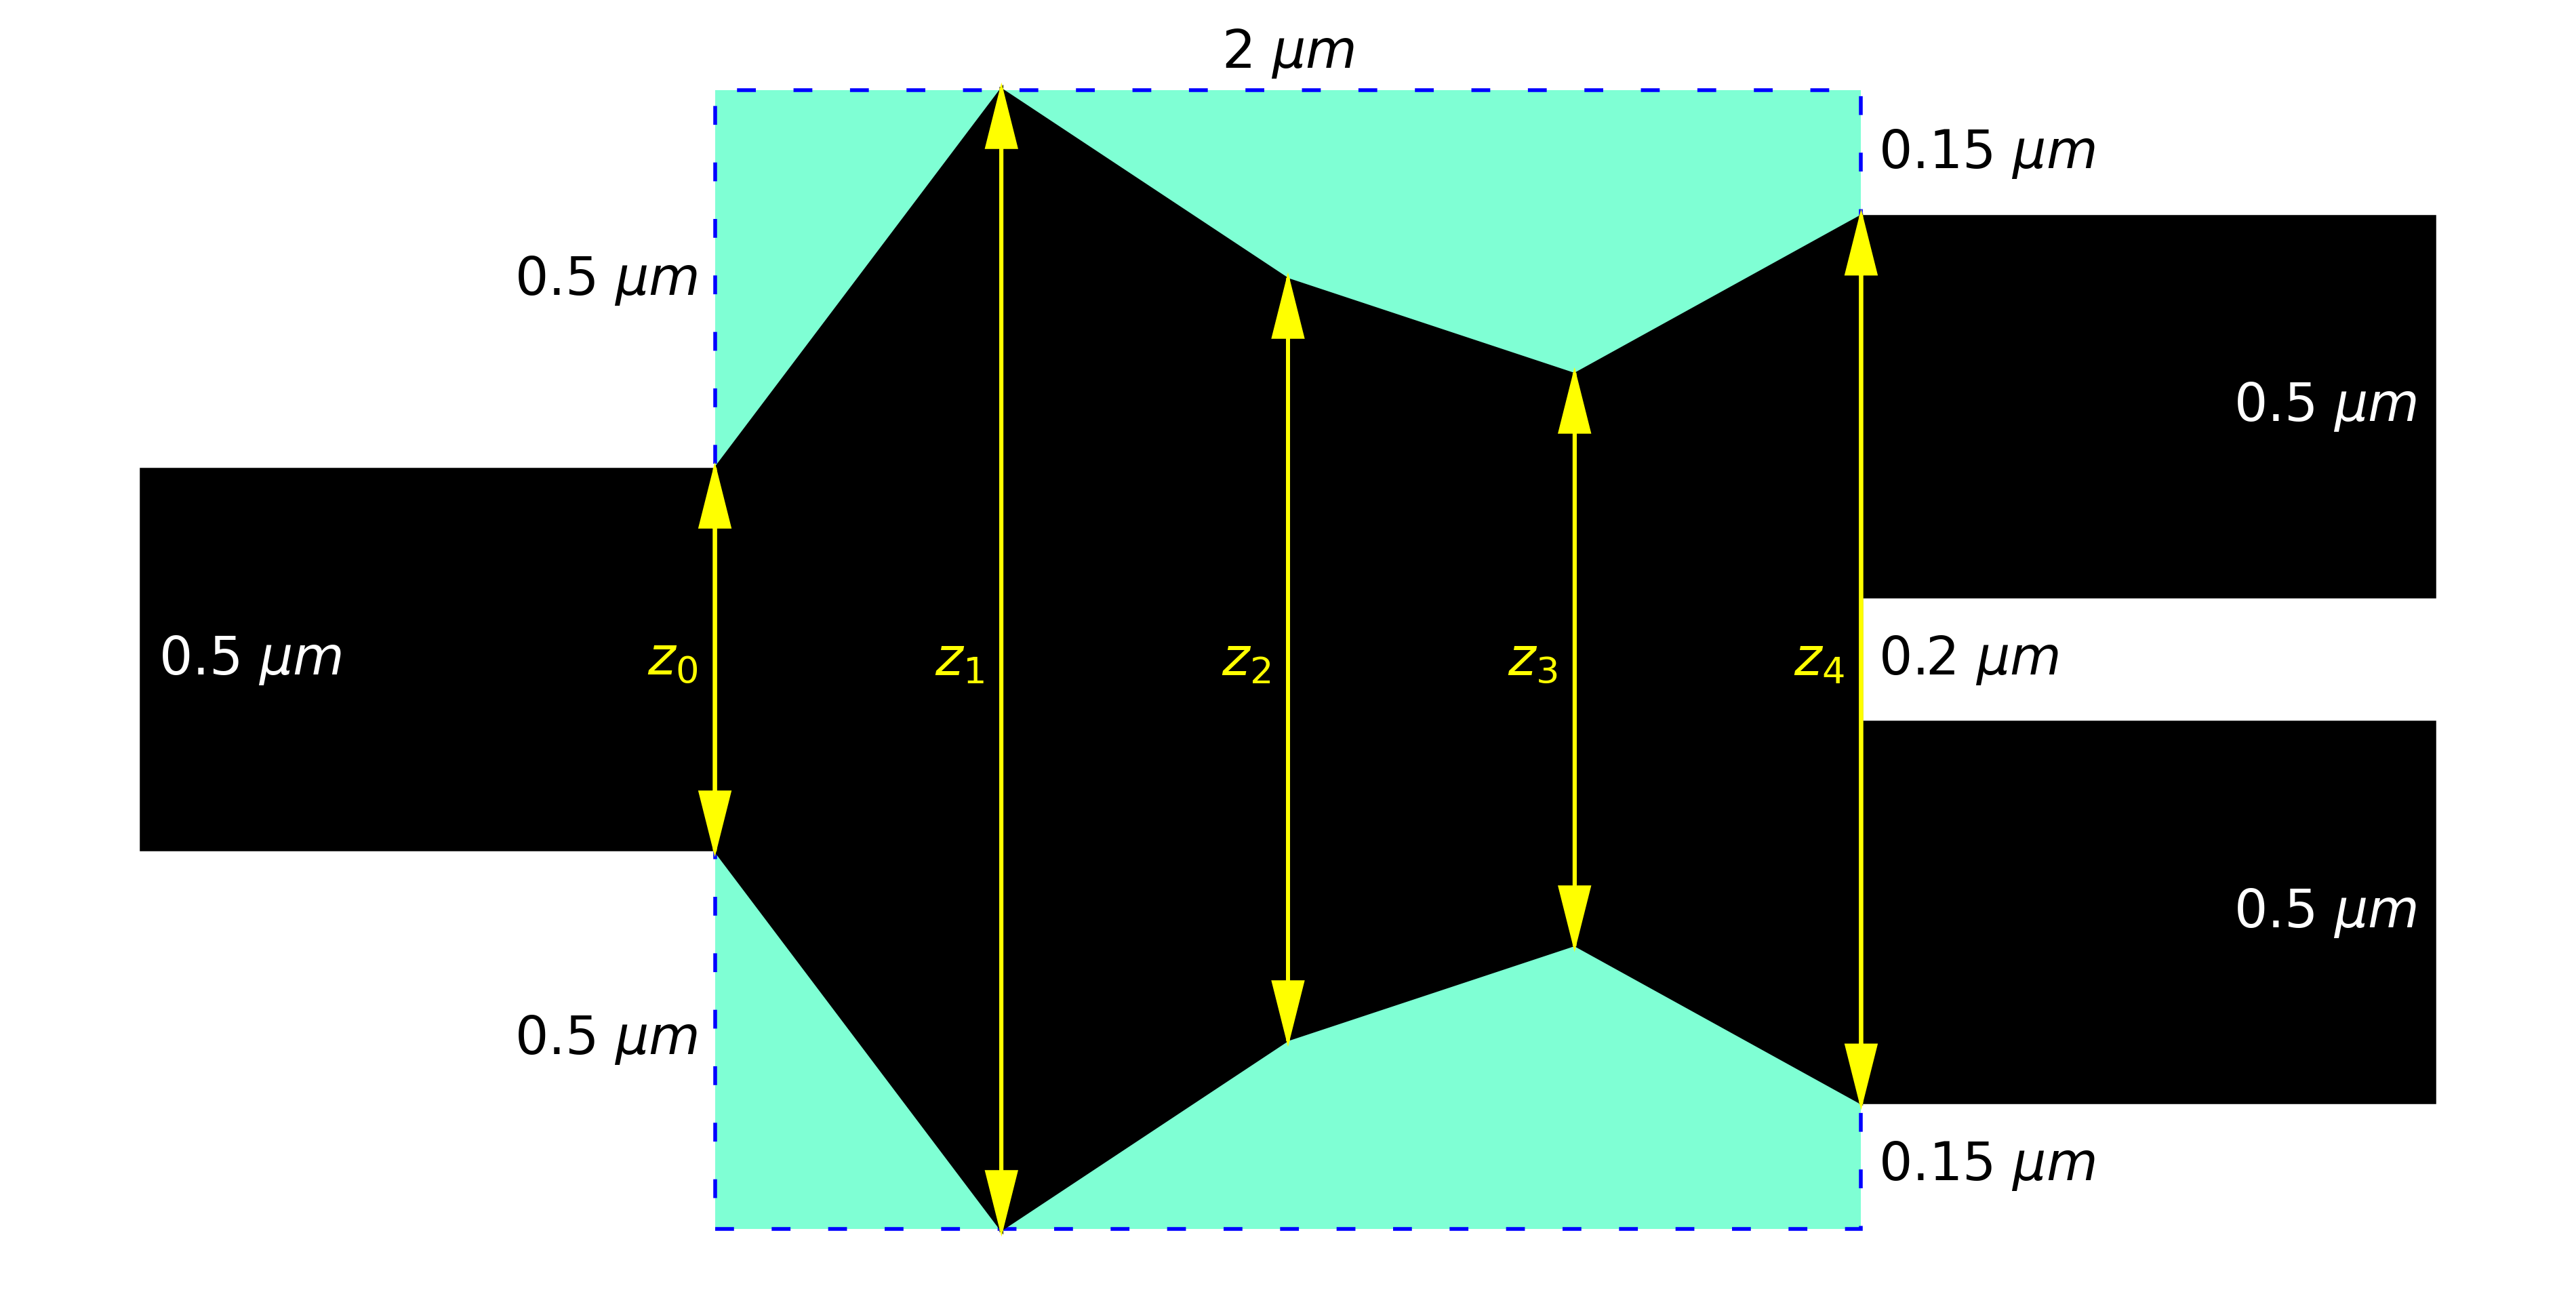
\includegraphics[scale=0.5]{image/related-works/mmi-angles.png}
  \caption{Diseño de un \emph{splitter} basado en \citep{Prosopio-Galarza2019} utilizando $z = 5$ segmentos.} 
  \label{fig:roy-mmi}
\end{figure}

Como función objetivo se establece maximizar la transmitancia en la guía de onda superior trabajando con una
longitud de onda de $1550 nm$.
Los mejores resultados son obtenidos al usar PSO como algoritmo de optimización.

Es destacable que al usar esta parametrización es posible limitar las alturas de los segmentos para asegurar 
obtener ángulos agudos, los cuales son los más adecuados como regla práctica de diseño
\citep{LukasChrostowski2010}.
Sin embargo, hay dos inconvenientes con este trabajo:

\begin{itemize}
  \item \textbf{Inconveniente 1:} 
  La parametrización utilizada descarta la posibilidad de diseños menos 
  intuitivos (por ejemplo, con agujeros) que podrían ocupar menor área y mantener una buena transmitancia.
  
  \item \textbf{Inconveniente 2:}
  Las optimizaciones solo se repitieron una vez con apenas 30 iteraciones y una población de 14 individuos.

\end{itemize}


A continuación, vamos a desarrollar en más detalle como otros trabajos han buscado solucionar estos dos inconvenientes.

\section{Inconveniente 1: La Parametrización}

Una estrategia de parametrización interesante es la de dividir de forma uniforme la región rectangular de diseño en 
$n \times m$ rectángulos como si fueran píxeles.
Luego, podemos considerar que un píxel negro representa la presencia de $Si$ y uno blanco de $SiO_2$,
como se mostró en la \autoref{fig:bend-discretization}.
Aunque trabajaron con otro dispositivo, esta estrategia se aplicó en \cite{Malheiros-Silveira2020} con $n
= m = 10$.

Sin embargo, una estrategia aún más interesante es la asignación a cada píxel de una permitividad
definida por la \autoref{eq:permitivity}, estrategia que se evaluó en \cite{Su2020} para optimizar un
\emph{bend} y \emph{WDM}. 
El principal beneficio de esta idea es que pasamos de tener un problema de optimización donde el resultado
solo podía tomar valores enteros a uno donde podemos considerar valores reales.
Con esto en consideración, se sigue la estrategia descrita en la \autoref{sec:estrategia-optimizacion}:
optimización continua y optimización discreta. 

Aún cuando la idea anterior es muy buena, al momento de incorporar restricciones de fabricación simplemente se
considera usar parámetros más grandes que la mínima precisión que puede manejar el equipo encargado de
fabricar el diseño.
Por otro lado, el trabajo presentado por \cite{Hammond20} brinda más detalles para esta etapa.
Lo más relevante de esta publicación es que a cada diseño le aplica transformaciones para simular la posible 
contracción o dilatación de estos al fabricarse.
Con lo anterior hace un intento de detectar estos dos errores de fabricación desde la etapa de optimización.

\section{Inconveniente 2: La Optimización}

En \cite{Malheiros-Silveira2020} se compararon dos algoritmos en la optimización de un dispositivo.
A diferencia de \cite{Prosopio-Galarza2019}, la comparación no se realizó en base a la cantidad de iteraciones
realizadas por cada algoritmo, en cambio se hizo de acuerdo a la cantidad de simulaciones realizadas 
($\approx 2000$), es decir, la cantidad de veces que se evaluó la FOM. 
Esta estrategia es más adecuada para comparar algoritmos con distintas características de una manera más justa.


En otros trabajos que se centran en comparar algoritmos para optimizar un mismo dispositivo se sigue la misma
idea para la comparación \citep{Schneider2019, Gregory2015}; sin embargo, no parece haber un consenso sobre algún algoritmo que funcione bien
para optimizar cualquier dispositivo.


En general, PSO y GA han sido extensamente usados en el área de acuerdo de acuerdo a reseñas como las de
\cite{Elsawy2020} y \cite{Campbell2019}. Tal y como es señalado en estos trabajos, el desempeño de ambos
algoritmos es sensible a los parámetros escogidos. Esta es un gran inconveniente debido a que escoger
parámetros adecuados puede consumir mucho tiempo y esto se debe hacer independientemente para cada
dispositivo. Con el propósito de superar esta dificultad, distintos trabajos están optando por usar algoritmos
que no necesiten configurar parámetros internos.


Bajo este enfoque, en \cite{Gregory2015} se resaltó el buen desempeño que pude obtener el algoritmo CMA-ES en
la optimización de ciertos dispositivos, llegando a superar al PSO.
De manera similar, en \cite{Schneider2019} se realizó un trabajo muy completo comparando distintos algoritmos
llegando a resultados donde la optimización bayesiana mostró los resultados más prometedores.
Y, aunque no entra en mucho detalle sobre la razón de esta elección, en \cite{Su2020} se empleó el algoritmo 
L-BFGS-B en la optimización de un \emph{bend} y WDM llegando a obtener resultados destacados.

Un aspecto importante a resaltar de estos últimos tres trabajos es que al comparar distintos algoritmos para
optimizar dispositivos fotónicos necesitamos contar con
(i) un elevado número de simulaciones y
(ii) distintas ejecuciones que comiencen con diferentes puntos iniciales.

Como se ha discutido en este capítulo, la parametrización de nuestros dispositivos usando un bajo número
de parámetros puede ir condicionando nuestros resultados, ante ellos podemos realizar una parametrización
más flexible basada en píxeles. Esto supone nuevos desafíos, mas ya existen estrategias para afrontarlos e
incluso para incluir restricciones de fabricación a esta parametrización.
Por otro lado, aunque no se mencionó explicítamente, no parece haber muchas
investigaciones que comparen distintos algoritmos cuando trabajamos con un elevado número de parámetros para
representar nuestros dispositivos, en especial si los algoritmos no son PSO o GA.
